%Version 3 October 2023 - Springer Nature Template
% Nature Communications submission

\documentclass[sn-nature]{sn-jnl}% Style for submissions to Nature Portfolio journals

%%%% Standard Packages
\usepackage{graphicx}%
\usepackage{multirow}%
\usepackage{amsmath,amssymb,amsfonts}%
\usepackage{booktabs}%
\usepackage{textcomp}%
\usepackage{siunitx}%
\usepackage{float}%
\usepackage{placeins}%

\raggedbottom

\begin{document}

\title[European Wind Energy Correlation]{The wind is always blowing somewhere in Europe: A decade of evidence for continental-scale renewable baseload}

%%=============================================================%%
%% Authors
%%=============================================================%%

\author*[1]{\fnm{Jan} \sur{Kren}}\email{jan.kren@psi.ch}

\author[2]{\fnm{Bo\v{s}tjan} \sur{Zajec}}\email{bostjan.zajec@cea.fr}

\author[3]{\fnm{Iztok} \sur{Tiselj}}\email{iztok.tiselj@fmf.uni-lj.si}

%%=============================================================%%
%% Affiliations
%%=============================================================%%

\affil*[1]{\orgdiv{Laboratory for Simulation and Modelling}, \orgname{Paul Scherrer Institute}, \orgaddress{\city{Villigen PSI}, \postcode{5232}, \country{Switzerland}}}

\affil[2]{\orgdiv{STMF/LE2H}, \orgname{CEA Paris-Saclay}, \orgaddress{\city{Gif-sur-Yvette}, \postcode{91191}, \country{France}}}

\affil[3]{\orgdiv{Faculty of Mathematics and Physics}, \orgname{University of Ljubljana}, \orgaddress{\city{Ljubljana}, \postcode{1000}, \country{Slovenia}}}

%%=============================================================%%
%% Abstract
%%=============================================================%%

\abstract{Wind power is intermittent at any single location---but it is always blowing somewhere across a continent. Here we test this premise using a decade of actual generation data from 29 European countries (2015--2024), the longest operational record analyzed to date. Unlike reanalysis-based studies, operational data capture curtailment, maintenance outages, and evolving fleet composition---effects invisible in simulated output. Aggregated European wind production never fell below \SI{5.5}{\giga\watt} (1.8\% of 2024 installed capacity), and geographic diversification reduced wind production variability by a stable $\sim$48\%. Yet Europe is failing to harness this potential. Although installed capacity doubled, the guaranteed baseload floor barely grew---a 2.1\% conversion rate---because new capacity concentrated in already-correlated Northwestern Europe rather than in weakly correlated regions like Iberia and Scandinavia. Adding solar raises the floor by 61\% and, more importantly, cuts battery storage costs by 81--93\%. These findings identify geographic diversification as a highly effective but largely untapped reliability mechanism for wind energy. Yet even under optimal siting, the wind baseload floor remains at just 3--5\% of installed capacity, covering only a small fraction of demand; a reliable zero-carbon grid requires wind alongside battery storage and firm clean generation.}

\keywords{wind energy, geographic diversification, baseload power, correlation analysis, energy policy}

\maketitle

%==============================================================================
\section{Introduction}\label{sec:intro}
%==============================================================================

Europe's energy transition rests on a massive expansion of variable renewables. Wind capacity alone has doubled from \SI{142}{\giga\watt} to \SI{300}{\giga\watt} in a decade\cite{windeurope2024}, solar has grown even faster, and EU targets call for more than 1,000~GW of wind by 2050. But variable generation poses a fundamental reliability question: what happens when the wind dies down and skies cloud over---not at one location, but across an entire continent? The answer hinges on a simple meteorological fact: weather is local. A blocking high over Germany can leave turbines idle from the North Sea to Bavaria while Atlantic storms drive strong generation across Iberia. The same high-pressure system that suppresses wind often brings clear skies, boosting solar. Geographic diversification---spreading capacity across regions with different weather---could, in principle, transform individually unreliable wind and solar into a collectively dependable portfolio. Whether this principle holds in practice, and whether Europe's expansion is exploiting it, are open questions.

Two decades of research support the premise. Spatial wind correlations decay exponentially with distance, with characteristic lengths of 400--1,000~km\cite{malvaldi2017,olauson2016,tong2021}, and even early Nordic studies showed that hourly variability drops substantially when production is aggregated across countries\cite{holttinen2005wind}. Portfolio-theoretic approaches confirm the benefit at European scale: geographic spreading reduces variability by 26\% in Markowitz-optimal portfolios\cite{lopezprol2024,roques2010,drake2007,markowitz1952}, and interconnected US wind farms could supply 33--47\% of output as baseload\cite{archer2007}. European wind synchronization is far from perfect, with correlation structures shaped by synoptic weather patterns\cite{monforti2016}. Large-scale atmospheric patterns---weather regimes, the North Atlantic Oscillation (NAO), blocking events---drive coherent multi-day swings in generation\cite{grams2017,brayshaw2011,bloomfield2020,vanderwiel2019weather}. Prolonged low-wind episodes (Dunkelflauten) are frequent at the country level but shorter and rarer at continental scale\cite{raynaud2018,kaspar2019,vanderwiel2019meteo}, though 38-year reanalysis studies have identified extreme events lasting weeks\cite{kittel2026}. Copula-based dependence models have been applied to wind power\cite{papaefthymiou2009,hagspiel2012}, with evidence that non-Gaussian copula families (Gumbel, Clayton) better capture joint extreme behavior\cite{louie2014}. A parallel body of work has established that wind and solar are naturally complementary: blocking highs that suppress wind bring clear skies, and their seasonal cycles are roughly anti-phased at European latitudes\cite{heide2010,huber2014,pfenninger2016}. Climate projections add urgency: under high-emission scenarios, more homogeneous wind patterns may intensify simultaneous shortfalls\cite{wohland_more_2017,qu2025}, making diversification even more critical.

Yet key questions remain unanswered. European studies---including the most comprehensive portfolio analysis to date\cite{lopezprol2024}---rely on reanalysis-derived capacity factors or simulated output (ERA5, Renewables.ninja\cite{staffell2016}); none has tracked diversification across a full decade of actual production, during which capacity doubled and the geographic distribution of turbines shifted substantially. It is therefore unknown whether the diversification benefit is stable over time, or whether the absolute reliability gain has kept pace with expansion. Operational data matter because reanalysis cannot capture curtailment, maintenance outages, evolving fleet composition, or the data-reporting artifacts documented by Hirth et al.\cite{hirth2018}. Critical metrics---such as the marginal baseload conversion rate (GW of guaranteed output per GW of installed capacity) and network densification trends (correlation structure evolving as the fleet grows)---require actual production records and cannot be derived from reanalysis snapshots. While wind-solar complementarity is well established in theory, it has not been quantified using operational data at the European scale. And the extreme tail structure---whether countries are more likely to hit simultaneous lows than linear correlations imply---has been examined for drought characterization\cite{otero2022copula}, but the spatial tail dependence of wind production has not been quantified systematically across the continent.

Here we address these gaps using the longest record of actual European renewable generation analyzed to date: hourly wind production from 29 countries and solar from 28 countries over 2015--2024, comprising approximately 87,600 hours of ENTSO-E operational data. We first quantify the pan-European baseload floor and its growth over the decade (Section~\ref{sec:results}). We then measure the diversification benefit and test its temporal stability using capacity-factor normalization (Section~\ref{sec:diversification}). The spatial correlation structure is examined to identify which regions drive the benefit, including scale-resolved analysis across timescales (Section~\ref{sec:diversification}). A greedy portfolio construction ranks countries by marginal diversification value. We assess regional versus pan-European reliability through cluster analysis, quantify the wind-solar complementarity and its impact on storage requirements (Section~\ref{sec:combined}), and characterize continental wind droughts using year-normalized thresholds alongside copula-based tail dependence analysis.


%==============================================================================
\section{Results}\label{sec:results}
%==============================================================================

\subsection{European wind never dropped to zero}

Aggregated European wind production never fell to zero in ten years of hourly observation. The 1st-percentile baseload---production exceeded 99\% of the time---is \SI{12.5}{\giga\watt} [95\% CI: 11.9--13.3~GW]. Even the absolute minimum never dropped below \SI{5.5}{\giga\watt} (1.8\% of 2024 installed capacity), a small but guaranteed and zero-carbon contribution (Table~\ref{tab:baseload}).

\begin{figure}[!ht]
    \centering
    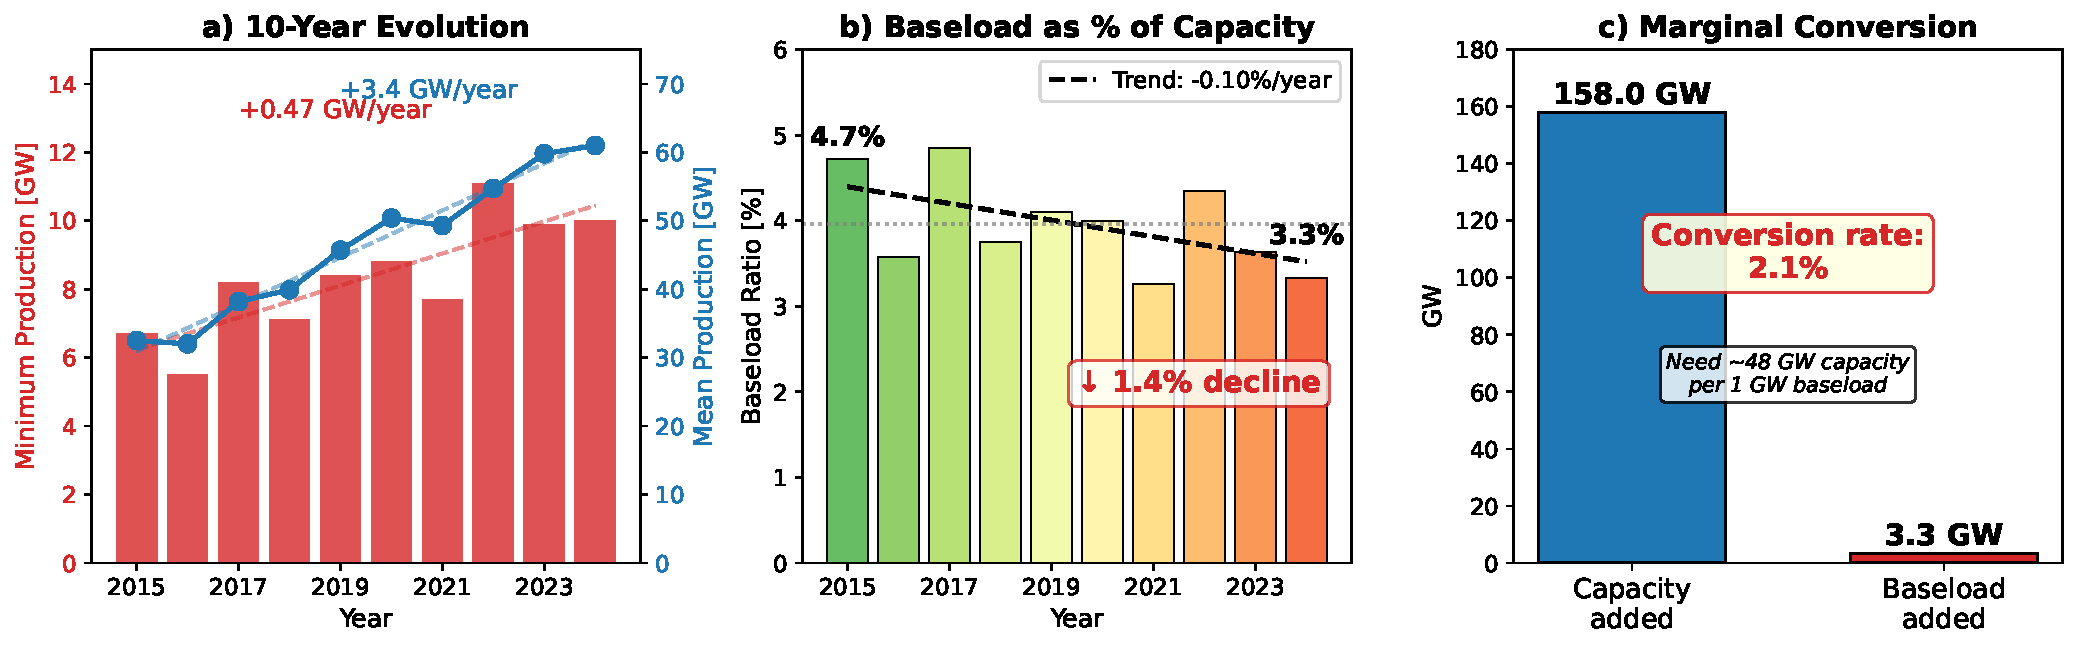
\includegraphics[width=\textwidth]{Figures_Paper/figure1_baseload.pdf}
    \caption{\textbf{European wind baseload analysis (2015--2024).} \textbf{a,} Ten-year evolution of minimum (baseload) and mean wind production. \textbf{b,} Baseload as percentage of installed capacity. \textbf{c,} Marginal conversion efficiency.}
    \label{fig:baseload}
\end{figure}

Yet this floor is growing disappointingly slowly (Fig.~\ref{fig:baseload}). Mean production and installed capacity both roughly doubled over the decade, but the baseload floor rose only 49\%---and as a fraction of installed capacity it actually fell, from 4.7\% to 3.3\% (Table~\ref{tab:baseload}). The marginal conversion rate is just 2.1\%: Europe needed $\sim$\SI{48}{\giga\watt} of new capacity for every \SI{1}{\giga\watt} of additional guaranteed output.

Relative to EU-27 mean electricity demand of $\sim$\SI{310}{\giga\watt} \cite{eurostat2024}, the wind baseload floor covers only 2--4\% of mean electricity demand---small in absolute terms, but guaranteed and zero-carbon. Winter baseload floors are higher (driven by stronger synoptic winds) but represent a smaller share of peak winter demand ($\sim$\SI{500}{\giga\watt}); adding solar (Section~\ref{sec:combined}) substantially raises the floor (by 61\% on average).

The contrast with individual countries explains why the floor exists at all. Germany, the largest producer, saw hourly output drop to effectively zero in 2024 (capacity factor $< 0.1\%$), yet the pan-European aggregate never fell below $\sim$10~GW that year. The sum of individual country minimums is nearly ten times lower than the aggregate minimum. Severe low-wind events (capacity factor $< 5\%$) simply do not occur simultaneously across a continent.

\begin{table}[!ht]
\centering
\caption{\textbf{Annual baseload statistics for aggregated European wind production.}}
\label{tab:baseload}
\begin{tabular}{lS[table-format=2.0]S[table-format=2.1]S[table-format=3.1]S[table-format=1.2]}
\toprule
Year & {Countries} & {Minimum [GW]} & {Mean [GW]} & {CV} \\
\midrule
2015 & 27 & 6.7 & 32.5 & 0.41 \\
2016 & 27 & 5.5 & 32.0 & 0.41 \\
2017 & 27 & 8.2 & 38.2 & 0.42 \\
2018 & 27 & 7.1 & 39.9 & 0.45 \\
2019 & 28 & 8.4 & 45.7 & 0.41 \\
2020 & 28 & 8.8 & 50.4 & 0.44 \\
2021 & 28 & 7.7 & 49.3 & 0.45 \\
2022 & 29 & 11.1 & 54.7 & 0.44 \\
2023 & 29 & 9.9 & 59.8 & 0.45 \\
2024 & 29 & 10.0 & 61.0 & 0.47 \\
\bottomrule
\end{tabular}
\end{table}


\subsection{Diversification halves variability---and the benefit is stable over time}
\label{sec:diversification}

Summing the individual minimum hourly outputs of all 29 countries yields only $\sim$0.5~GW---nearly ten times less than the pan-European aggregate minimum shown in Table~\ref{tab:baseload}. The gap arises because national low-wind hours rarely coincide: imperfect correlation between wind regimes across the continent means one country's trough is another's average. We quantify this smoothing effect using the coefficient of variation, $\text{CV} = \sigma/\mu$, which measures the relative dispersion of hourly production within a calendar year, where $\sigma$ is the standard deviation and $\mu$ the mean. Because CV is dimensionless, it can be compared across countries and years regardless of installed capacity, making it the natural metric for tracking diversification as the fleet evolves.

The \textit{diversification benefit} (DB) quantifies how much geographic aggregation reduces variability:
\begin{equation}
    \text{DB} = \frac{\overline{\text{CV}}_{\text{countries}} - \text{CV}_{\text{aggregate}}}{\overline{\text{CV}}_{\text{countries}}} \times 100\%
    \label{eq:db}
\end{equation}
where $\overline{\text{CV}}_{\text{countries}} = \frac{1}{N}\sum_{i=1}^{N} \text{CV}_i$ is the unweighted mean over $N$ countries. A DB of 100\% would imply that aggregation eliminates all relative variability (perfectly uncorrelated national wind regimes), while a DB of 0\% would mean the aggregate is no smoother than the average country (fully synchronized wind across Europe). Over the decade, DB averaged $\sim$48\%, meaning aggregation nearly halves relative variability (Fig.~\ref{fig:diversification}).

\begin{figure}[!ht]
    \centering
    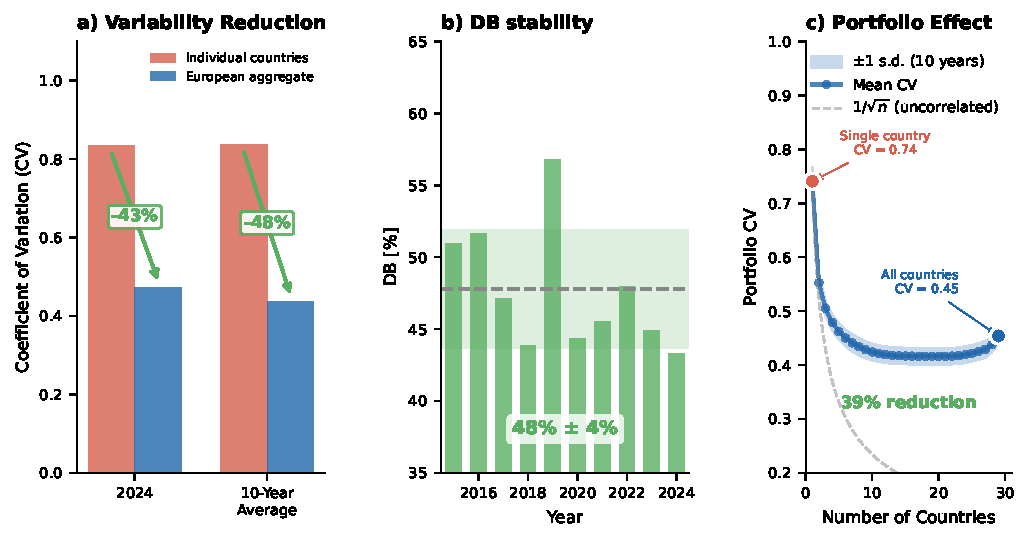
\includegraphics[width=\textwidth]{Figures_Paper/figure2_diversification.pdf}
    \caption{\textbf{Diversification benefit analysis.} \textbf{a,} Mean individual country CV versus aggregated European CV; the gap is the diversification benefit. \textbf{b,} Annual diversification benefit ($47.8 \pm 4.3$\%), stable throughout the decade despite capacity doubling. \textbf{c,} Portfolio effect: CV decreases as countries are added in greedy order (Table~\ref{tab:marginal}). Shaded band shows $\pm$1~s.d.\ across years; the curve remains above the $1/\sqrt{n}$ line for uncorrelated sources, reflecting positive spatial correlations.}
    \label{fig:diversification}
\end{figure}

The diversification benefit averaged $47.8 \pm 4.3$\% (mean $\pm$ s.d.) across the decade---stable despite capacity nearly doubling, two countries joining the analysis, and a major shift toward offshore wind. (The 2019 value of 57\% is an outlier driven by Slovakia's negligible wind fleet entering the unweighted average with an anomalous CV; excluding Slovakia yields $46.4 \pm 3.0$\%.) While the aggregate CV itself rose slightly (Table~\ref{tab:baseload}), reflecting growing concentration of capacity in correlated regions, individual country CVs rose in parallel, leaving DB unchanged. This stability suggests the benefit is a property of European wind climatology, not an artifact of any particular capacity distribution. Two alternative formulations confirm this robustness (Supplementary Table~4): a production-weighted DB (which gives larger producers more influence) and a capacity-factor-normalized DB (using capacity factor $= \bar{P}/P_{\text{installed}}$ instead of raw MW). The production-weighted DB averages 38\% and the CF-normalized DB 45\%, both tracking the unweighted value (48\%) across all ten years, confirming that the diversification benefit is meteorological rather than an artifact of weighting or capacity growth.

The diversification benefit varies with the seasons (Supplementary Fig.~1). Summer has lower production but stronger diversification (DB~$= 57.7\%$), because localized, thermally driven winds are less correlated across countries than winter's large-scale synoptic systems. Winter reverses the pattern: higher production, weaker DB (47\%). This matters for reliability, because weaker diversification coincides with peak electricity demand---the highest-risk periods combine high load with correlated production dips across broad regions.

Adding solar reshapes the seasonal picture. In winter, DB rises modestly from 47\% to 50\%, reflecting solar's limited output. In summer, however, the combined wind+solar DB (40\%) is \textit{lower} than wind-only (54\% for the subset of countries with both wind and solar data)---because the synchronized daily solar cycle across Europe adds correlated variability that is harder to diversify away than wind's stochastic fluctuations. The higher absolute production of the combined portfolio (56~GW vs 31~GW mean) more than compensates. Combined portfolios provide year-round reliability, but through different mechanisms: wind-solar complementarity in winter, production volume in summer.


\subsection{Correlation structure reveals where to build next}

The 48\% DB (Sec.~\ref{sec:diversification}) depends on imperfect spatial correlations. We now examine this structure to identify which regions drive the benefit and where further investment would yield the greatest returns (Fig.~\ref{fig:map}).

\begin{figure}[!ht]
    \centering
    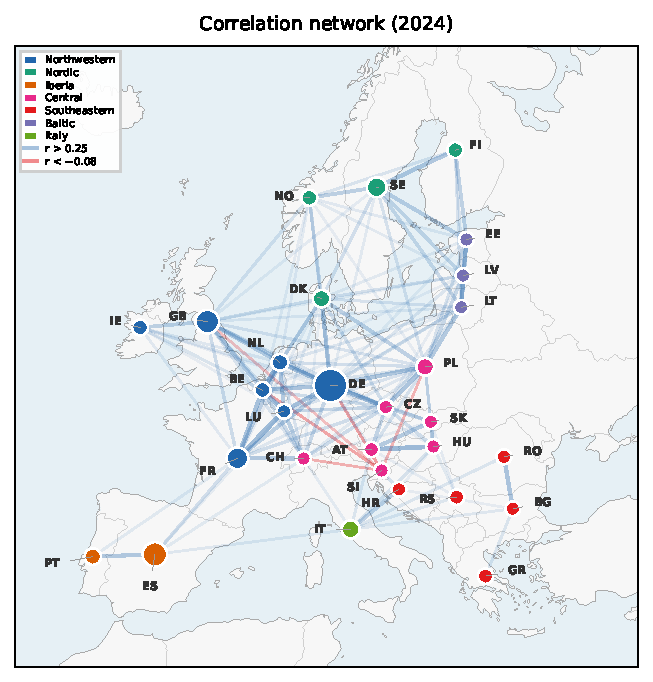
\includegraphics[width=\textwidth]{Figures_Paper/figure3_map.pdf}
    \caption{\textbf{Geographic structure of European wind correlations (2024).} Correlation network: nodes represent countries (sized by mean production, colored by regional cluster). Blue edges show positive correlations ($r > 0.25$), red edges negative correlations ($r < -0.08$); edge width is proportional to $|r|$. Of the 406 possible pairs, 173 are shown.}
    \label{fig:map}
\end{figure}

Five regional correlation clusters emerge from the pairwise correlation analysis (Fig.~\ref{fig:map}). Northwestern Europe (Belgium, Netherlands, Germany, Luxembourg, France, UK) is tightly correlated, with Belgium--Netherlands reaching $r = 0.89$ in 2024 ($r = 0.85$ averaged over the decade). The Nordic countries and Central Europe form moderately correlated clusters, while Iberia shows strong internal correlation but weak coupling to the rest of the continent. Notably, Southeastern Europe shows negative correlations with the Northwest: when wind is low in Germany, it tends to be elevated in Serbia.

To examine how correlations depend on timescale, we bandpass-filtered each country's hourly production at logarithmically spaced periods (8~h to 60~days) and computed the Pearson correlation of the filtered signals (see Methods). The resulting scale-resolved analysis (Fig.~\ref{fig:scale_resolved}) reveals strong scale dependence: adjacent pairs (e.g., Belgium--Netherlands) remain correlated at all timescales ($r > 0.4$), while distant pairs (e.g., Portugal--Finland) show near-zero correlation regardless of scale. The separation grows with timescale and is already pronounced at synoptic scales (2--7 days), confirming that geographic diversification acts primarily on the weather-scale fluctuations that dominate day-to-day variability.

\begin{figure}[!ht]
    \centering
    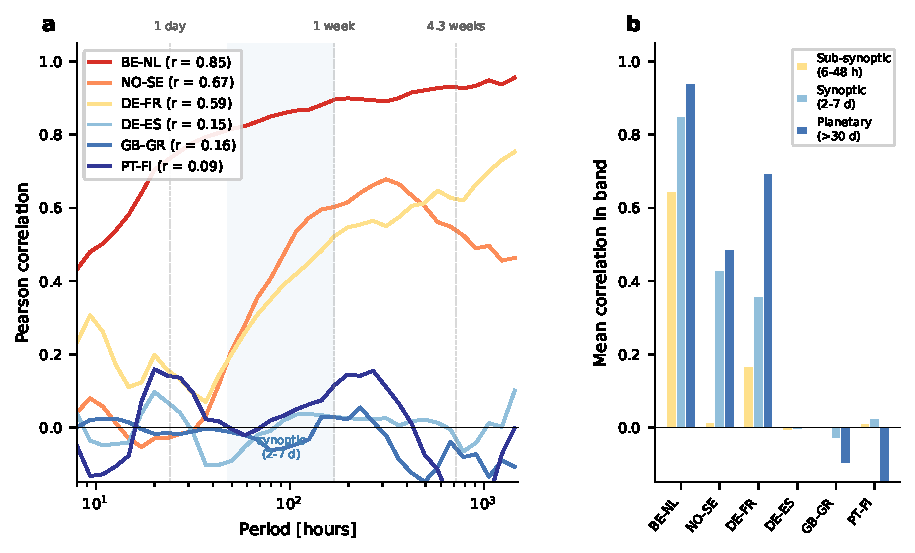
\includegraphics[width=\textwidth]{Figures_Paper/figure_wavelet_coherence.pdf}
    \caption{\textbf{Scale-resolved correlation analysis of selected country pairs (2015--2024).} \textbf{a,} Pearson correlation of bandpass-filtered wind production (one-octave bandwidth) as a function of period for six representative country pairs spanning high-correlation (Belgium--Netherlands, $r=0.85$; Norway--Sweden, $r=0.67$), moderate-correlation (Germany--France, $r=0.59$), and low-correlation (Germany--Spain, $r=0.15$; Great Britain--Greece, $r=0.16$; Portugal--Finland, $r=0.09$) regimes. The shaded band marks synoptic timescales (2--7~days). Adjacent countries remain strongly correlated at all timescales ($r > 0.4$), while distant pairs show near-zero correlation regardless of scale. \textbf{b,} Band-averaged correlation for three canonical timescale bands: sub-synoptic (6--48~h), synoptic (2--7~d), and planetary ($>$30~d). The separation between nearby and distant pairs grows monotonically with timescale.}
    \label{fig:scale_resolved}
\end{figure}

Not all countries contribute equally. Greedy portfolio construction (a sequential algorithm that adds at each step the country minimizing portfolio CV; Table~\ref{tab:marginal}; Supplementary Fig.~2) reveals that, starting from Germany, adding Spain provides the greatest marginal benefit, followed by Sweden and Italy---the top five span four distinct climate zones. This ranking is robust to the choice of starting country (Supplementary Fig.~5, Supplementary Table~3). Northwestern European countries actually \textit{increase} portfolio CV when added last, because their tight correlation with Germany adds variability faster than production. EU priority projects should emphasize north-south corridors and connections to Southeastern Europe, rather than reinforcing the Northwestern cluster.

\begin{table}[!ht]
\centering
\caption{\textbf{Countries ranked by marginal diversification value (2015--2024).} Starting from Germany, each successive country is added by the greedy algorithm to minimize portfolio CV.}
\label{tab:marginal}
\begin{tabular}{llS[table-format=1.3]l}
\toprule
Rank & Country & {Cumulative CV} & Region \\
\midrule
1 & Germany & 0.731 & Northwestern \\
2 & Spain & 0.562 & Iberian \\
3 & Sweden & 0.519 & Nordic \\
4 & Italy & 0.494 & Southern \\
5 & Greece & 0.480 & Mediterranean \\
6 & Portugal & 0.469 & Iberian \\
7 & Ireland & 0.461 & Northwestern \\
8 & Romania & 0.454 & Southeastern \\
9 & Norway & 0.448 & Nordic \\
10 & Finland & 0.444 & Nordic \\
\bottomrule
\end{tabular}
\end{table}

This geographic picture is evolving over time (Supplementary Fig.~3). Network density---the fraction of country pairs with $|r| > 0.3$---rose from 0.22 (2015) to 0.26 (2024), an 18\% increase, while the number of distinct correlation clusters (identified by the Louvain community detection algorithm~\cite{blondel2008}) fell from 8 to 4. European wind production is becoming more spatially correlated, likely because offshore expansion in the North Sea concentrates capacity where Belgium, Netherlands, Germany, Denmark, and the UK already share synoptic patterns. If this densification continues as offshore wind scales toward 300~GW by 2050~\cite{windeurope2024}, future DB may fall below today's levels---unless policy deliberately directs capacity toward weakly correlated regions.


\subsection{Pan-European integration delivers a 2.5-fold reliability dividend}

How much does continental integration improve reliability compared to isolated regional grids? We computed baseload floors for seven regional groups (distinct from the correlation clusters above) reflecting Europe's synchronous zones and grid topology: Northwestern Europe (DE, NL, BE, FR, LU, GB, IE), Nordic (NO, SE, DK, FI), Iberia (ES, PT), Central Europe (AT, CH, CZ, SK, HU, PL, SI), Southeastern Europe (RO, BG, GR, RS, HR), Baltics (EE, LV, LT), and Italy (Fig.~\ref{fig:regional}).

\begin{figure}[!ht]
    \centering
    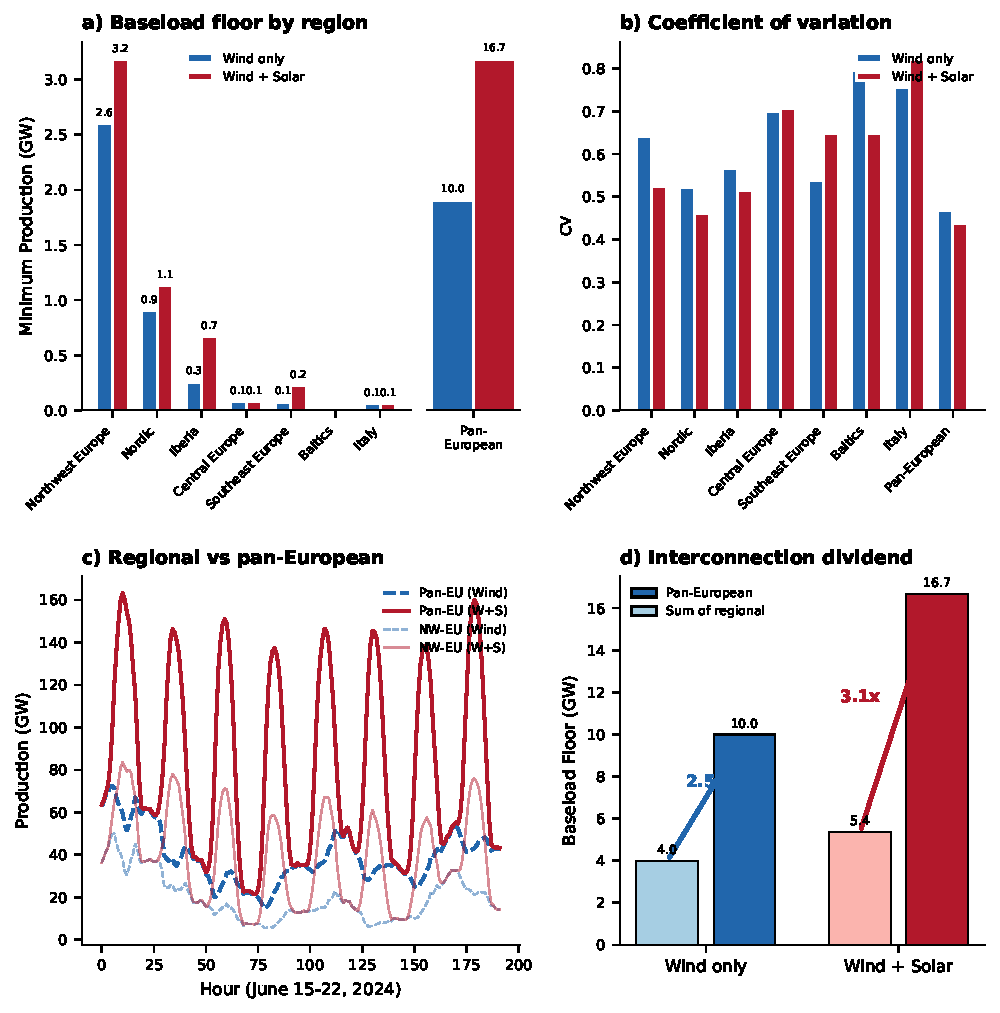
\includegraphics[width=\textwidth]{Figures_Paper/figure_regional_clustering.pdf}
    \caption{\textbf{Regional versus pan-European baseload floors (2024).} \textbf{a,} Minimum production by region comparing wind-only (blue) versus combined wind+solar (red). Pan-European bars (right axis) are shown on a separate scale to illustrate the aggregation benefit. \textbf{b,} CV by region. \textbf{c,} Hourly time series (June 15--22, 2024) for the full pan-European aggregate (thick) and Northwestern Europe (thin, faded): wind-only (dashed blue) versus combined wind+solar (solid red). \textbf{d,} Interconnection dividend: the ratio of pan-European baseload floor to the sum of regional floors---2.5$\times$ for wind-only, 3.1$\times$ for combined wind+solar.}
    \label{fig:regional}
\end{figure}

The sum of regional wind-only minimums---what Europe could guarantee if each cluster operated in isolation---is only $\sim$4~GW. The pan-European minimum is 2.5$\times$ higher (Fig.~\ref{fig:regional}d). The mechanism is weak inter-regional correlation: Northwestern Europe correlates moderately with Central and Nordic regions, but weakly with Iberia and Southeastern Europe. When Northwestern production falls to its bottom 5\%, Southeastern Europe produces \textit{above} its annual average; when Iberian production crashes, the rest of Europe produces at normal levels.

Adding solar amplifies the dividend. The pan-European combined minimum rises to nearly 17~GW, boosting the interconnection dividend from 2.5$\times$ to 3.1$\times$. Southern regions contribute strong solar that complements northern wind patterns, while smaller regions like Central Europe and the Baltics would face severe challenges in isolation. The 2.5--3.1$\times$ dividend is an upper bound: transmission constraints, loop flows, and political barriers would reduce the realized benefit. Building new interconnectors is costly and contentious---Germany's long-delayed north-south lines illustrate the challenge even within a single country. Nevertheless, the mechanism is clear: when one region's wind production falls, another's compensates, and only interconnection can exploit this.


\subsection{Adding solar raises the floor by 61\% and slashes storage costs}
\label{sec:combined}

Wind and solar are natural complements: the high-pressure systems that suppress wind often bring clear skies\cite{heide2010,huber2014}. We find a European-aggregate wind-solar Pearson correlation of $r = -0.26$ over the full decade (computed from all hourly data including nighttime hours, when solar generation is zero)---the first such estimate from operational data at continental scale (Fig.~\ref{fig:combined}).

\begin{figure}[!ht]
    \centering
    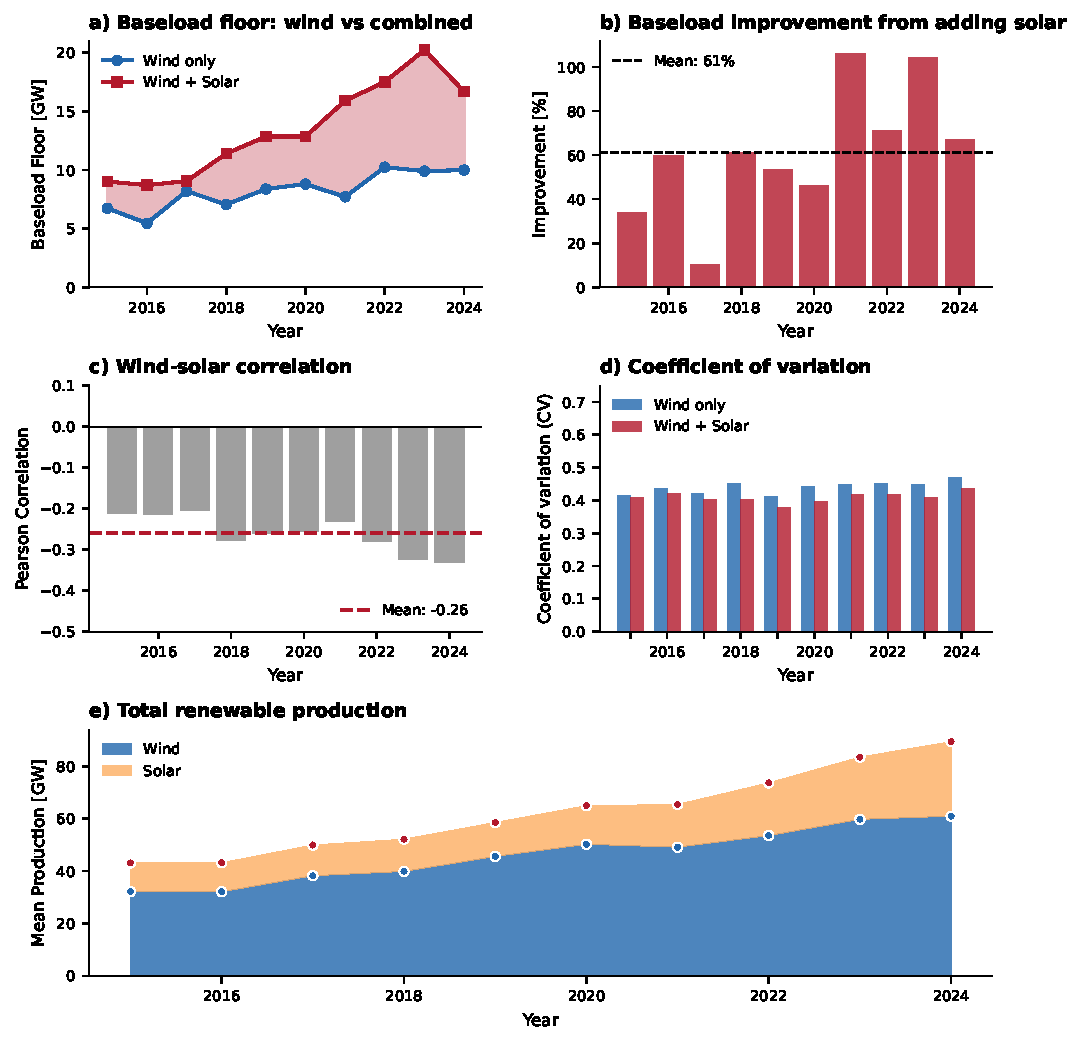
\includegraphics[width=\textwidth]{Figures_Paper/figure_combined_wind_solar.pdf}
    \caption{\textbf{Combined wind and solar baseload analysis.} \textbf{a,} Baseload floor comparison: combined wind+solar (red) versus wind-only (blue), showing consistent improvement across the decade. \textbf{b,} Baseload improvement from adding solar, defined as (combined min $-$ wind min) / wind min $\times$ 100\%; decade mean 61\% (range: 11--106\%). \textbf{c,} Aggregate wind-solar Pearson correlation by year, demonstrating stable negative correlation ($r \approx -0.26$) confirming complementarity. \textbf{d,} Annual CV comparison showing modest additional smoothing from the combined portfolio. \textbf{e,} Mean annual production growth, with wind (blue) and solar (orange) contributions shown as stacked areas.}
    \label{fig:combined}
\end{figure}

Adding solar increased the European baseload floor by 61\% on average (Supplementary Table~2), raising the 2024 minimum from \SI{10.0}{\giga\watt} to \SI{16.7}{\giga\watt}. At the country level, 24 of 27 countries show negative wind-solar correlation, with the strongest complementarity at high latitudes where summer solar peaks coincide with the wind trough. Continental aggregation captures additional inter-country complementarity: the aggregate correlation ($r = -0.26$) is stronger than the mean country-level value ($r = -0.11$).

The combined portfolio modestly reduces variability, but the real payoff appears in storage requirements (Supplementary Fig.~4, Supplementary Table~1). At current utility-scale lithium-ion costs \cite{bnef2024battery}, adding solar reduces the battery storage needed to guarantee a given baseload floor by an order of magnitude---81--93\% savings across target wind+solar+battery baseload floors of 20 to 40~GW---because solar generates during many low-wind hours, reducing both the frequency and duration of deficits. These costs assume 100\% coverage of the target floor over the entire decade; real deployments targeting 99.9\% reliability would need substantially less. Our combined estimates are conservative because ENTSO-E solar data captures only $\sim$83\% of official EU generation \cite{eurostat2024}, with the gap concentrated in distributed rooftop systems.


\subsection{Continental wind droughts are rare---but tail risks warrant caution}

Grid planners must consider worst cases: prolonged continent-wide calm, or \textit{Dunkelflauten} (literally ``dark doldrums,'' referring to periods without both wind and solar). Although the term strictly implies the absence of both sources, we follow Kittel and Schill~\cite{kittel2026} in applying the multi-threshold framework to wind-only production---effectively characterizing continental wind droughts---at three severity levels (Fig.~\ref{fig:dunkelflaute}).

\begin{figure}[!ht]
    \centering
    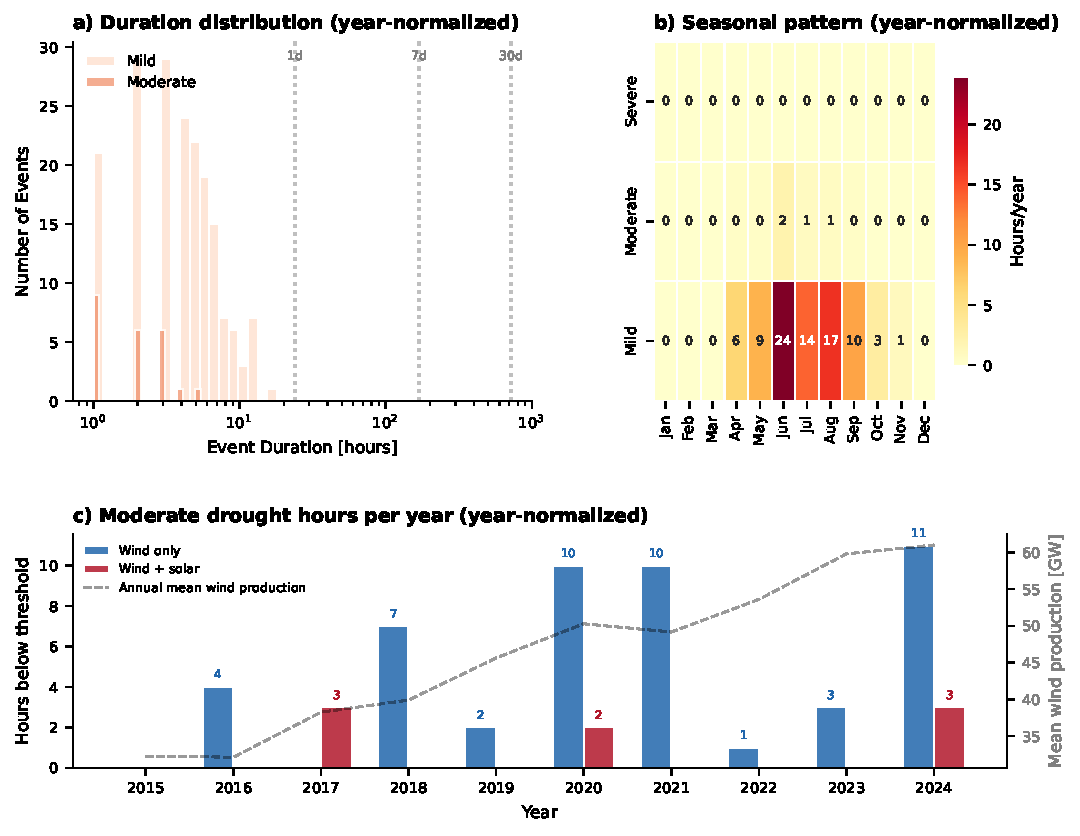
\includegraphics[width=\textwidth]{Figures_Paper/figure3_dunkelflaute.pdf}
    \caption{\textbf{Pan-European wind drought analysis (2015--2024), year-normalized thresholds.} \textbf{a,} Event duration distribution by severity level (thresholds relative to each year's mean). \textbf{b,} Seasonal distribution of moderate events (hours per year). \textbf{c,} Moderate drought hours per year for wind only (blue; threshold at 20\% of annual mean wind) and combined wind+solar (red; threshold at 20\% of annual mean wind+solar). Adding solar eliminates most moderate drought hours, particularly in summer. The dashed line shows rising annual mean wind production.}
    \label{fig:dunkelflaute}
\end{figure}

Because installed capacity nearly doubled over the decade, we use year-normalized thresholds---defined relative to each year's own mean production---to separate genuine meteorological changes from the mechanical effect of capacity growth (see Methods).

No \textbf{severe wind drought} (production below 10\% of that year's mean) occurred at the continental scale during the entire ten years (Fig.~\ref{fig:dunkelflaute}a). This contrasts sharply with individual countries: Germany alone had 860 hours below its own 20\% threshold in 2024. This contrast is the diversification benefit in action: individual countries experience severe droughts, but continental aggregation smooths them out.

\textbf{Moderate wind droughts} (below 20\% of year mean) persist throughout the decade, with the longest single event lasting 5 hours and events clustering in summer and early autumn when synoptic forcing is weakest (Fig.~\ref{fig:dunkelflaute}a,b). Notably, 2024 recorded the most moderate hours (11~h), confirming that continental wind droughts have not diminished despite the doubling of installed capacity (Fig.~\ref{fig:dunkelflaute}c). The minimum-to-mean ratio shows no improving trend (0.21 in 2015, 0.16 in 2024; Table~\ref{tab:baseload}), meaning geographic diversification has not reduced the relative depth of continental wind droughts, even as absolute production floors rise with capacity. Adding continental solar production to the portfolio reduces moderate drought hours from 48 to 8 over the decade (83\%; Fig.~\ref{fig:dunkelflaute}c), because solar peaks in the summer months when wind droughts are most frequent.

But do countries synchronize more during extremes, eroding diversification when it matters most? Standard (Pearson) correlations measure average co-movement; they cannot detect whether countries become \textit{more} correlated specifically when production is very low. Tail dependence analysis addresses this directly: the lower tail dependence coefficient $\lambda_L$ (range 0--1) measures the probability that two countries are simultaneously in their lowest production percentiles. A value of zero would mean extreme lows are independent; a value of one would mean they always coincide (Fig.~\ref{fig:tail}).

\begin{figure}[!ht]
    \centering
    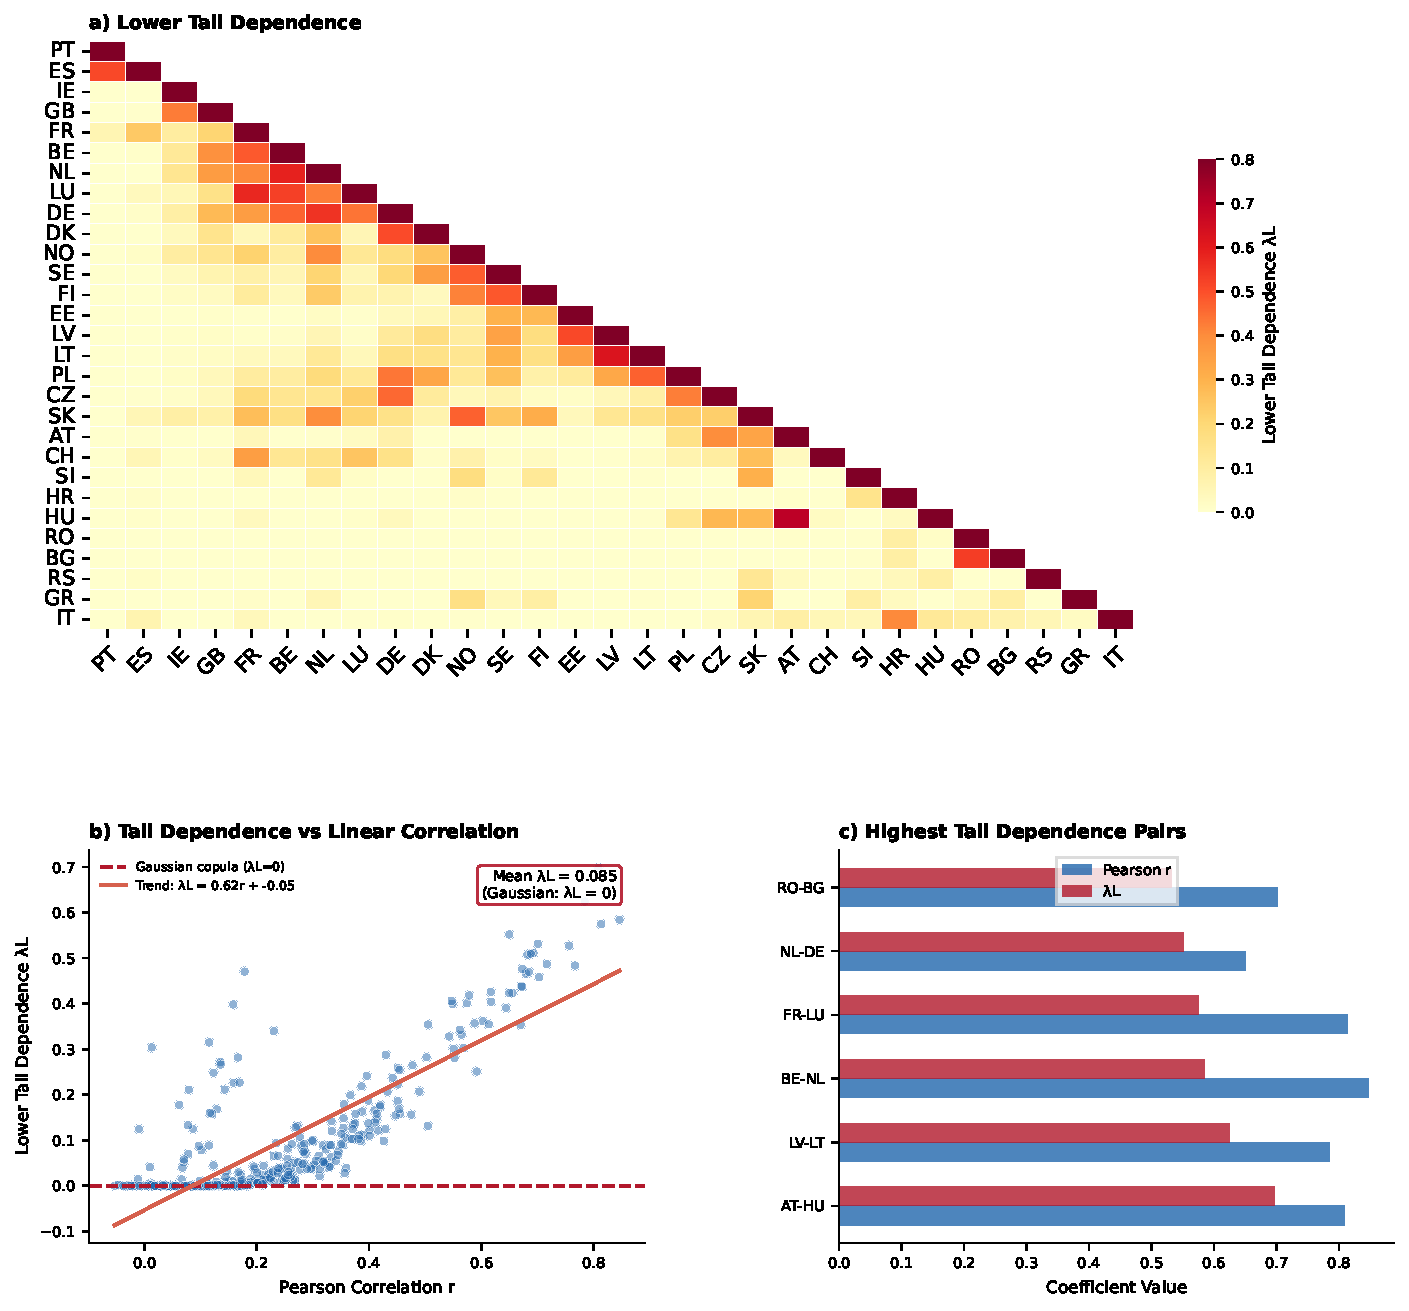
\includegraphics[width=\textwidth]{Figures_Paper/figure5_tail_dependence.pdf}
    \caption{\textbf{Tail dependence analysis.} \textbf{a,} Lower tail dependence ($\lambda_L$) heatmap showing spatial clustering of extreme co-occurrence. \textbf{b,} Relationship between Pearson correlation and tail dependence, with Gaussian reference ($\lambda_L = 0$); mean $\lambda_L = 0.085$ across 406 pairs. \textbf{c,} Comparison of Pearson correlation and lower tail dependence for the six highest-dependence pairs: Austria--Hungary (0.70), Latvia--Lithuania (0.62), Belgium--Netherlands (0.58).}
    \label{fig:tail}
\end{figure}

We find a mean $\lambda_L$ of 0.085 across all country pairs---small but non-zero, meaning countries are somewhat more likely to hit simultaneous lows than average correlations alone would predict. The effect is concentrated among immediate neighbors (e.g., Austria--Hungary reaches 0.70; Fig.~\ref{fig:tail}a,c). At this level, diversification still delivers 80--90\% of the benefit that a model assuming independent extremes would predict, and the high-dependence pairs are countries already known to be tightly correlated.

An important caveat: our 10-year record cannot characterize events with multi-decadal return periods. Kittel and Schill~\cite{kittel2026}, using 38 years of ERA5 reanalysis, found a 55-day European Dunkelflaute in winter 1996/97---outside our observation window. Our finding complements rather than contradicts reanalysis studies: the absence of severe events in 87,600 operational hours provides empirical grounding, but does not preclude longer events in the past or future.


%==============================================================================
\section{Discussion}\label{sec:discussion}
%==============================================================================

Our central finding is that Europe's wind baseload floor is real, robust, and growing---but growing too slowly. We use ``baseload floor'' not to claim wind is dispatchable, but to emphasize that the aggregated output of 29 countries never reached zero---a statistical property with practical consequences for capacity planning.

The low conversion rate is not a physical limit; it reflects where Europe chose to build. Most new capacity went to Germany, Denmark, and the Netherlands---countries already tightly correlated. Spain, Sweden, and Italy would each yield far greater baseload per GW installed, because their wind regimes are weakly correlated with the existing fleet. The stable DB reinforces this: expansion concentrated in already-represented regions left the correlation structure unchanged. As Europe targets 510~GW by 2030 and over 1,000~GW by 2050~\cite{windeurope2024}, whether the floor grows proportionally depends on \textit{where} new capacity is sited, not just how much.

Our operational findings are broadly consistent with the simulation literature but add empirical grounding. The smoothing benefit aligns with L\'opez Prol et al.'s~\cite{lopezprol2024} Markowitz-optimal portfolios (26\% CV reduction using Renewables.ninja data), though magnitudes differ due to metric differences and the distinction between simulated and operational output. Comparison with Kittel and Schill's~\cite{kittel2026} 38-year Dunkelflaute study illustrates the complementary value of production and reanalysis data: their longer record captures events outside our window, while our data captures operational realities invisible to reanalysis.

The policy implication is direct: Europe must diversify \textit{where} it builds, not merely \textit{how much}. The 2.5-fold interconnection dividend (3.1-fold with solar) quantifies what geographic breadth delivers---consistent with model-based cooperation benefits \cite{schlachtberger2017,rodriguez2014}. North-south corridors and connections to Southeastern Europe should take priority over reinforcing the already-dense Northwestern cluster. Realizing this potential faces political barriers: Norway's recent interconnector restrictions illustrate that cross-border integration is as much a political question as a technical one. Network densification over the decade warns that continued concentration of offshore capacity in the North Sea could erode DB. Offshore wind farms exhibit higher spatial correlation than onshore \cite{kempton2010,potisomporn2022,hjelmeland2023}; this concentration effect demands deliberate countermeasures through geographically distributed deployment.

A key limitation of our interconnection dividend is the assumption of unconstrained transmission. In practice, cross-border flows are limited by net transfer capacities (NTCs), and practical limits are well below nominal values due to loop flows and security constraints \cite{entsoe2024tyndp}. Our regional analysis suggests that equalizing production across clusters during low-wind hours requires inter-regional transfers of $\sim$15--20~GW---within nominal corridor capacity but requiring near-simultaneous use of multiple corridors. The ENTSO-E TYNDP 2024 plans $\sim$\texteuro328~billion in grid reinforcement by 2040; our results suggest that prioritizing corridors connecting weakly correlated regions would maximize the reliability dividend per euro invested.

Yet even optimally diversified wind leaves a large gap. A baseload floor of 3--5\% of installed capacity means the vast majority of demand must be met by other means. Combined wind-solar portfolios help---the wind-solar anticorrelation raised the floor by 61\% and cut storage costs by over 80\%---but the seasonal mismatch is stubborn: winter combines peak demand with the lowest DB and weakest solar contribution, when firm backup is most needed. Multi-week periods during which continental production remains below any practical baseload target (e.g., 20--40~GW) are visible in our data and exceed the reach of battery storage. Geographic diversification, solar complementarity, short-duration storage, and firm zero-carbon baseload generation are complements, not alternatives \cite{brown2018}; a reliable decarbonized grid requires all four.

Important limitations temper these conclusions. Our 10-year record, while the longest operational analysis to date, cannot characterize events with multi-decadal return periods. ENTSO-E data have documented quality issues \cite{hirth2018}: wind reporting is relatively complete, but solar data captures only $\sim$83\% of official EU generation, with substantial undercounting of distributed systems, making our combined estimates conservative. Adding the missing distributed solar would increase the combined baseload floor by an estimated 10--15\%. The interconnection dividend is an upper bound: transmission constraints, loop flows, and market barriers would reduce the realized benefit. Climate change introduces further uncertainty: projections of more homogeneous European wind fields under warming \cite{wohland_more_2017,tobin2015} would intensify simultaneous shortfalls, drought durations may lengthen by $\sim$15\% \cite{qu2025}, and temporally compounding droughts across wind, solar, and hydropower pose systemic risks beyond single-technology analyses \cite{vandermost2024}. Our decade-long baseline provides a reference against which such shifts can be detected.

Notwithstanding these caveats, a decade of operational data establishes three facts. First, aggregated European wind production never fell to zero---the 1st-percentile baseload is \SI{12.5}{\giga\watt} (4.2\% of 2024 installed capacity), and even the absolute minimum never dropped below \SI{5.5}{\giga\watt} (1.8\%). Second, geographic diversification is the mechanism: aggregating 29 countries nearly halved relative variability (DB~$= 47.8 \pm 4.3$\%), and this benefit was stable despite capacity doubling and the offshore share surging. Third, Europe is not exploiting this advantage. The 2.1\% marginal conversion rate is not a physical ceiling; it is the consequence of concentrating expansion in already-correlated Northwestern European countries.

The solution lies in where capacity is built, not how much. Spain, Sweden, and Italy each offer an order of magnitude more marginal diversification value than additional capacity in Germany or the Netherlands. Pairing wind with solar raises the baseload floor by 61\% and cuts storage requirements by over 80\%. Pan-European interconnection delivers a 2.5-fold reliability dividend over isolated regional grids---rising to 3.1-fold when solar is included. These gains require investment in north-south transmission corridors and cross-regional interconnectors, not reinforcement of already-saturated clusters.

Yet even optimal diversification cannot close the gap alone. A baseload floor of 3--5\% of installed capacity leaves the vast majority of demand to be met by other means. The seasonal mismatch---winter peak demand coinciding with the lowest DB and weakest solar---demands firm zero-carbon generation for multi-week deficits that no plausible battery deployment can bridge. Geographic diversification, solar complementarity, short-duration storage, and firm dispatchable generation are complementary, not competing, strategies.

The wind is always blowing somewhere in Europe. Whether that meteorological fact translates into energy security depends on where we build, how we connect, and what we pair it with.


%==============================================================================
\section{Methods}\label{sec:methods}

\subsection{Data sources and processing}

We obtained hourly wind generation data from the ENTSO-E Transparency Platform for 28 European countries, supplemented by UK data from the Elexon BMRS API (post-June 2021, following Brexit-related reporting gaps), for a total of 29 countries covering January 2015 to December 2024: Austria (AT), Belgium (BE), Bulgaria (BG), Switzerland (CH), Czech Republic (CZ), Germany (DE), Denmark (DK), Estonia (EE), Spain (ES), Finland (FI), France (FR), Great Britain (GB), Greece (GR), Croatia (HR), Hungary (HU), Ireland (IE), Italy (IT), Lithuania (LT), Luxembourg (LU), Latvia (LV), Netherlands (NL), Norway (NO), Poland (PL), Portugal (PT), Romania (RO), Serbia (RS), Sweden (SE), Slovenia (SI), and Slovakia (SK). Croatia and Serbia have partial coverage beginning in 2018 and 2021 respectively. The ENTSO-E Transparency Platform has known data quality limitations \cite{hirth2018}; wind reporting is relatively complete for most countries, though Netherlands onshore wind is partially underreported (only farms connected directly to TenneT appear in the data).

Raw data were processed by: (1) normalizing timestamps to UTC; (2) summing Wind Onshore and Wind Offshore generation; (3) resampling to hourly means for cross-country alignment; (4) identifying common timestamps across all countries within each year; and (5) linearly interpolating gaps up to 3 hours. The final dataset comprises approximately 87,600 hourly observations.

Installed capacity values for capacity-factor normalization were obtained from WindEurope annual statistics reports, ranging from 142~GW (2015) to 300~GW (2024, estimated). These are end-of-year totals; actual capacity varies within years as new installations are commissioned. Repeating the correlation analysis with $\pm$10\% capacity perturbations changed mean pairwise correlations by less than 0.01, confirming robustness.

Solar PV generation data were obtained from the ENTSO-E Transparency Platform for 28 countries over the same period and processed identically to wind data. ENTSO-E reporting captures only utility-scale and large commercial installations; by comparing 2023 ENTSO-E totals against Eurostat official statistics, we estimate coverage at approximately 83\% of total EU solar generation. The gap is concentrated in countries with high distributed solar shares---most notably the Netherlands, where ENTSO-E captures only $\sim$3\% of actual solar generation. Our combined wind-solar baseload estimates are therefore conservative.

\subsection{Variability and diversification metrics}

The coefficient of variation (CV) and diversification benefit (DB) are defined in Section~\ref{sec:diversification}, Eq.~\ref{eq:db}. We use an unweighted mean over countries because it treats each country as a potential diversification source regardless of current capacity, consistent with the forward-looking question of where to build next. Supplementary Table~4 confirms that production-weighted and capacity-factor-normalized (capacity factor $= \bar{P}/P_{\text{installed}}$) variants yield similar magnitudes (38--45\% vs.\ 48\%), indicating that DB is a robust property of European wind climatology rather than an artifact of any particular weighting.

Percentile-based baseload measures complement the absolute minimum, which can be sensitive to single outlier hours. We report the 1st and 5th percentiles of hourly production across the decade, with confidence intervals estimated using block bootstrap (200 resamples, block size 168 hours) to preserve temporal autocorrelation.

\subsection{Correlation analysis and network structure}

Pearson correlation coefficients were computed for all 406 country pairs. Confidence intervals used the Fisher z-transformation with effective sample size correction for autocorrelation \cite{bayley1946}:
\begin{equation}
    n_{\text{eff}} = \frac{n}{1 + 2\sum_{k=1}^{K} \rho_{xx}(k)}
\end{equation}
where $\rho_{xx}(k)$ is the autocorrelation at lag $k$, summed until $\rho < 2/\sqrt{n}$. Multiple testing correction used the Benjamini-Hochberg procedure at $\alpha = 0.05$.

Correlation networks were constructed for each year with countries as nodes and edges for pairs with $|r| > 0.3$ (results are qualitatively robust to thresholds between 0.2 and 0.4). Network density is the fraction of possible edges present: $D = 2E / (N(N-1))$, where $E$ is the edge count and $N = 29$ countries. Community detection used the Louvain algorithm \cite{blondel2008} with correlation weights.

\subsection{Marginal diversification analysis (greedy algorithm)}

We quantified the marginal value of each country using greedy portfolio construction over the full decade. Hourly wind production from all available countries was concatenated across years, yielding approximately 50,800 common hours across 28 countries (Serbia excluded due to incomplete temporal overlap). Starting with Germany (the largest producer), we iteratively added the country $i$ that maximized $\Delta\text{CV}_i = \text{CV}_{\text{current}} - \text{CV}_{\text{current} + i}$, continuing until all countries were included. Countries present in fewer than 5 years were excluded. The ranking is sensitive to the starting country; Germany was chosen as it represents $\sim$40\% of European wind production. Sensitivity analysis starting from France, Spain, and the UK confirms that Spain, Sweden, Italy, and Greece remain in the top five regardless of starting point (Supplementary Table~3).

\subsection{Regional clustering analysis}

Countries were grouped into seven regional clusters reflecting geographic proximity and grid topology: Northwestern Europe (DE, NL, BE, FR, LU, GB, IE), Nordic (NO, SE, DK, FI), Iberia (ES, PT), Central Europe (AT, CH, CZ, SK, HU, PL, SI), Southeastern Europe (RO, BG, GR, RS, HR), Baltics (EE, LV, LT), and Italy. For each region, we computed hourly aggregate production and extracted the minimum over 2024. The ``interconnection dividend'' is the ratio of the pan-European minimum to the sum of regional minimums. This analysis was performed for both wind-only and combined wind+solar portfolios.

\subsection{Combined wind-solar analysis}

For each year, wind and solar generation were aggregated independently: wind across all countries with sufficient data ($>$7,000 valid hours that year), and solar likewise. A country contributed its wind generation even if it lacked solar data, and vice versa. Valid timestamps were defined as hours with data from all selected wind countries and all selected solar countries; the combined portfolio production at each hour is their sum. The number of wind countries ranges from 27 (2015--2018) to 29 (2022--2024); solar countries range from 19 (2016) to 25 (2024), reflecting the progressive rollout of ENTSO-E solar reporting. UK solar data from ENTSO-E ends mid-2021 due to post-Brexit reporting changes; we supplemented this with Elexon BMRS API data through 2024. Serbia solar data is unavailable throughout. The baseload improvement factor is defined as (combined minimum $-$ wind minimum) / wind minimum $\times$ 100\%.

\subsection{Battery storage requirements}

For each target floor level $F$, the hourly deficit is $D(t) = \max(0, F - P(t))$ where $P(t)$ is actual production. Required power capacity is $\max_t D(t)$; required energy capacity is $E = \max_{[t_1,t_2]} \int_{t_1}^{t_2} D(t)\,\mathrm{d}t$ over all contiguous shortfall periods $[t_1, t_2]$, representing the deepest discharge cycle. Cost estimates used \$150/kWh for energy capacity and \$200/kW for power capacity, representing a lower-bound projection for 4-hour utility-scale lithium-ion systems. These values fall below the NREL ATB 2024 Moderate scenario (\$326/kWh total system cost for 2030) \cite{nrel2024} but are consistent with recent Chinese LFP market benchmarks. The percentage savings from adding solar are robust to cost assumptions: at \$300/kWh, savings shift from 81--93\% to 82--94\%.

\subsection{Wind drought event detection}

Following Kittel and Schill\cite{kittel2026}, we defined Dunkelflaute events using three severity thresholds applied to pan-European aggregate production: severe ($<$10\% of mean), moderate ($<$20\%), and mild ($<$30\%). We used \textit{year-normalized thresholds} based on each year's own mean production, which isolate meteorological variability from the confounding effect of capacity growth. Because installed capacity nearly doubled over the decade, a fixed absolute threshold would show spuriously vanishing droughts even if relative drought severity were unchanged. We used mean production rather than installed capacity as the normalizing variable because hourly installed capacity is not reported in ENTSO-E data; annual mean production serves as a proxy that captures the net effect of capacity additions, retirements, and evolving capacity factors. An event consists of consecutive hours below the threshold, with a 6-hour gap merging nearby episodes. Reported durations include both below-threshold and intervening gap hours, reflecting the total period over which backup capacity would need to remain available.

\subsection{Copula-based tail dependence}

We estimated tail dependence by fitting Clayton copulas to each country pair. The Clayton copula captures lower tail dependence---the tendency for countries to experience simultaneous low production---which is the critical concern for energy security. The Gumbel copula, which Louie~\cite{louie2014} found provides the best overall fit for wind power dependence, captures upper tail dependence (simultaneous high production), which is less relevant here.

Data were first transformed to uniform marginals using the empirical cumulative distribution function. The Clayton copula is:
\begin{equation}
    C(u,v) = (u^{-\theta} + v^{-\theta} - 1)^{-1/\theta}
\end{equation}
with parameter $\theta > 0$ estimated by maximum likelihood. The lower tail dependence coefficient is $\lambda_L = 2^{-1/\theta}$ (for the Gaussian copula, $\lambda_L = 0$ regardless of correlation). To validate our copula choice, we performed Cram\'er-von Mises goodness-of-fit tests comparing Clayton, Gumbel, and Gaussian copulas on all 406 pairs. Mean CvM statistics are nearly identical across families (0.0012--0.0013), and Clayton-derived $\lambda_L$ values correlate well with nonparametric estimates ($r = 0.72$), confirming that our conclusions are not an artifact of copula choice.

\subsection{Seasonal and scale-resolved analysis}

Seasons were defined as winter (December--February), spring (March--May), summer (June--August), and autumn (September--November). CV and DB were computed separately for each season using the same methodology as the annual analysis.

Scale-resolved correlations (Fig.~\ref{fig:scale_resolved}) were computed as follows: for each center period $T$ (logarithmically spaced from 8~h to 60~days), both country time series were bandpass-filtered using a third-order Butterworth filter with one-octave bandwidth ($T/\sqrt{2}$ to $T\sqrt{2}$), and the Pearson correlation of the filtered signals was computed over the full decade. Each point on the $r(T)$ curve in Fig.~\ref{fig:scale_resolved}a thus represents the linear correlation between two countries at a specific timescale. Edge transients (10\% on each side) were discarded. This approach isolates the meteorological co-variation at each timescale without the smoothing artifacts that cause time-averaged wavelet coherence to converge toward unity at long periods.

All analyses were performed in Python 3.9 using NumPy 1.24, SciPy 1.11, pandas 2.0, statsmodels 0.14, and NetworkX 3.1. Code and processed data are available at \url{https://github.com/JanKren/Renewable-Baseload}.


%==============================================================================
\backmatter
%==============================================================================

\bmhead{Data availability}

The analysis code and processed datasets are available at \url{https://github.com/JanKren/Renewable-Baseload} and archived on Zenodo (DOI: 10.5281/zenodo.XXXXXXX).% TODO: Replace XXXXXXX with actual Zenodo DOI before submission
Raw data can be obtained from the ENTSO-E Transparency Platform (\url{https://transparency.entsoe.eu}) and Elexon BMRS (\url{https://bmrs.elexon.co.uk}).

\bmhead{Code availability}

All analysis code is available at \url{https://github.com/JanKren/Renewable-Baseload} under the MIT License.

\bmhead{Acknowledgements}

We thank ENTSO-E for making Transparency Platform data publicly available, and Elexon for providing UK generation data via the BMRS API.

\bmhead{Author contributions}

J.K.\ and B.Z.\ conceived the study. J.K.\ developed the methodology, obtained and processed the data, performed the analysis, and wrote the manuscript. B.Z.\ contributed to methodology development, validated the statistical analysis, and revised the manuscript. I.T.\ contributed to methodology development and revised the manuscript. All authors discussed the results and contributed to the final version.

\bmhead{Competing interests}

The authors declare no competing interests.


%%===========================================================================================%%
%% References - using sn-nature bibliography style
%%===========================================================================================%%

\bibliography{references1}


\end{document}
